
% This LaTeX was auto-generated from MATLAB code.
% To make changes, update the MATLAB code and republish this document.

\documentclass{article}
\usepackage{graphicx}
\usepackage{color}

\sloppy
\definecolor{lightgray}{gray}{0.5}
\setlength{\parindent}{0pt}

\begin{document}

    
    
\subsection*{Contents}

\begin{itemize}
\setlength{\itemsep}{-1ex}
   \item c) Simulaci�n de VA usando el m�todo de la transformada inversa
   \item d)
\end{itemize}


\subsection*{c) Simulaci�n de VA usando el m�todo de la transformada inversa}

\begin{verbatim}
clc,close all
% numero de puntos
N=10000;
% simular una variable aleatoria uniforme
X = rand(N,1);
%  simular una variable exponencial con el metodo de la transformada inversa
k = 2/9; Y = sqrt(2.*X./k);
h = hist(Y,100);
% normalizar el histograma
% h = h / sum(h);   bar(h);   legend('show'); title('Histograma de pdf');
% print('-depsc',[dir 'histograma_c']);
\end{verbatim}


\subsection*{d)}

\begin{verbatim}
close all
% clase 4 ej 4pkg load statistics
rand('seed',1234);
% numero de realizaciones de la v.a.
N = 1e4;
% simulaciones de la variable independiente
n = 1e4;
% variable independiente
x = linspace(-1,4,n);
% constante de filtrado (y dispersion de la Gaussiana)
h = 0.05;
% Igualo lo encontrado en el punto anterior con la X a estimar
X=Y;
%  pdf estimada
p = zeros(size(x));
% para cada muestra
for i=1:N
    % para cada variable independiente
    for j=1:length(x)
        % kernel function, Gaussian
        K = (1/sqrt(2*pi))*exp(-(1/2)*((X(i)-x(j))/h)^2);
        % estimation of pdf
        p(j) = p(j) + (1/(N*h)) * K;
    end;
end;
plot(x,p)
grid on
print('-depsc',[dir 'kernel']);
\end{verbatim}

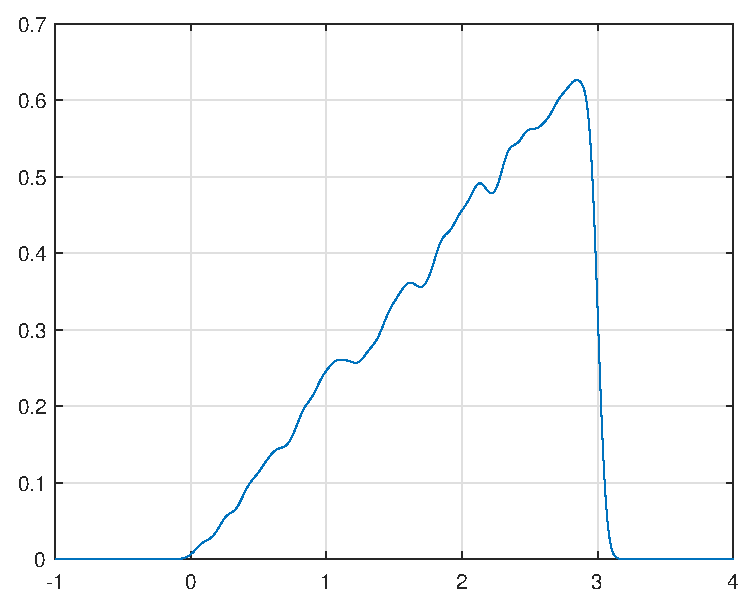
\includegraphics [width=4in]{ej_2_examen_01.eps}



\end{document}
    
